\documentclass[usenames,dvipsnames]{beamer}

\usefonttheme{serif}
\setbeamertemplate{items}[circle]
\setbeamertemplate{footline}[frame number]

\usepackage{pxfonts}
\usepackage{mathpazo}
\usepackage{tcolorbox}
\usepackage{soul}
\usepackage{algorithm,algorithmic}
\usepackage{geometry}

\beamertemplatenavigationsymbolsempty

\DeclareMathOperator*{\minimize}{minimize}
\DeclareMathOperator*{\Exp}{\mathbf{E}}
\DeclareMathOperator{\Regret}{Regret}
\DeclareMathOperator{\Reward}{Reward}
\DeclareMathOperator{\Risk}{Risk}
\DeclareMathOperator{\polylog}{polylog}
\DeclareMathOperator*{\argmin}{argmin}
\DeclareMathOperator*{\argmax}{argmax}

\newcommand{\R}{\mathbb{R}}
\newcommand{\indicator}{\mathbf{1}}
\newcommand{\norm}[1]{\left\|#1\right\|}
\newcommand{\KL}[2]{KL\left({#1}\middle\|{#2}\right)}
\newcommand{\grad}{\nabla}
\newcommand{\Breg}{\mathcal{B}}

\newcommand{\Cite}[1]{{\tiny \textcolor{Blue}{[#1]}}}

\makeatletter
\newcommand\SoulColor{%
\let\set@color\beamerorig@set@color
\let\reset@color\beamerorig@reset@color}
\makeatother
\setstcolor{red}


\title{Parameter-Free and Scale-Free \\ Online Algorithms}

\date{November 9, 2016}
\author{Francesco Orabona \and D\'avid P\'al}
\institute{Stony Brook University \\ \& \\ Yahoo Research, New York}

\begin{document}

%%%%%%%%%%%%%%%%%%%%%%%%%%%%%%%%%%%%%%%%%%%%%%%%%%%%%%%%%%%%%%%%%%%%%%%%%%%%%%%%%%%%%%%%%%
\begin{frame}
\maketitle
\end{frame}

%%%%%%%%%%%%%%%%%%%%%%%%%%%%%%%%%%%%%%%%%%%%%%%%%%%%%%%%%%%%%%%%%%%%%%%%%%%%%%%%%%%%%%%%%%
\begin{frame}
\frametitle{Online Linear Optimization}

Given a convex set $K \subseteq \R^N$

\vspace{0.3cm}

For $t=1,2,\dots$
\begin{itemize}
\item predict $w_t \in K$
\item receive loss vector $\ell_t \in \R^N$
\item suffer loss $\langle \ell_t, w_t \rangle$
\end{itemize}

\pause
\vspace{0.3cm}
$$
\Regret_T(u) = \textcolor{ForestGreen}{\underbrace{\sum_{t=1}^T \langle \ell_t, w_t \rangle}_{\text{algorithm's loss}}} \ - \ \textcolor{red}{\underbrace{\sum_{t=1}^T \langle \ell_t, u \rangle}_{\text{competitor's loss}}}
$$

\pause
\vspace{0.3cm}

Examples:
\begin{enumerate}
\item $K = \R^N$
\item $K = \Delta_N = \{ x \in \R^N ~:~ x \ge 0, \norm{x}_1 = 1 \}$
\end{enumerate}

\end{frame}

%%%%%%%%%%%%%%%%%%%%%%%%%%%%%%%%%%%%%%%%%%%%%%%%%%%%%%%%%%%%%%%%%%%%%%%%%%%%%%%%%%%%%%%%%%
\begin{frame}
\frametitle{FTRL and MD}

\begin{center}
\fontsize{7pt}{8}\selectfont
\begin{tabular}{c|c}
Follow The Regularized Leader & Mirror Descent \\ \hline
\begin{minipage}{0.45\linewidth}
\vspace{0.1cm}
\begin{algorithmic}
{
\STATE Initialize $L_0 \leftarrow 0$
\FOR{$t=1,2,3,\dots$}
\STATE Choose a regularizer $R_t:K \to \R$
\STATE $w_t \leftarrow \argmin_{w \in K} \langle L_{t-1}, w \rangle + R_t(w)$
\STATE Predict $w_t$
\STATE Observe $\ell_t \in V^*$
\STATE $L_t \leftarrow L_{t-1} + \ell_t$
\ENDFOR
}
\end{algorithmic}
\vspace{0.1cm}
\end{minipage}
&
\begin{minipage}{0.45\linewidth}
\vspace{0.1cm}
\begin{algorithmic}
{
\STATE Choose a regularizer $R_0:K \to \R$
\STATE $w_1 \leftarrow \argmin_{w \in K} R_0(w)$
\FOR{$t=1,2,3,\dots$}
\STATE Predict $w_t$
\STATE Observe $\ell_t \in V^*$
\STATE Choose a regularizer $R_t:K \to \R$
\STATE $w_{t+1} \leftarrow \argmin_{w \in K} \langle \ell_t, w \rangle + \Breg_{R_t}(w, w_t)$
\ENDFOR
}
\end{algorithmic}
\vspace{0.1cm}
\end{minipage}
\end{tabular}
\end{center}

\pause
\vspace{1cm}

\fontsize{8pt}{8}\selectfont

\begin{align*}
FTRL: \qquad \Regret_T(u) & \le R_{T+1}(u) + R_1^*(0) + \sum_{t=1}^T \Breg_{R_t^*}(-L_t, -L_{t-1}) - R_t^*(-L_t) + R_{t+1}^*(-L_t) \\
MD: \qquad \Regret_T(u) & \le \sum_{t=1}^T \langle \ell_t, w_{t} - w_{t+1} \rangle - \Breg_{R_t}(w_{t+1}, w_t) + \Breg_{R_t}(u, w_{t}) - \Breg_{R_t}(u, w_{t+1})
\end{align*}

\end{frame}

%%%%%%%%%%%%%%%%%%%%%%%%%%%%%%%%%%%%%%%%%%%%%%%%%%%%%%%%%%%%%%%%%%%%%%%%%%%%%%%%%%%%%%%%%%
\begin{frame}
\frametitle{FTRL/MD Bound}

\begin{theorem}[\textcolor{Blue}{CBL'06, SS'11}]
Let $R:K \to \R$ be a non-negative $1$-strongly convex w.r.t. $\norm{\cdot}$. \\
FTRL and MD with regularizer $R_t(w) = \frac{1}{\eta} R(w)$ satisfies
$$
\forall u \in K \qquad  \Regret_T(u) \le \frac{R(u)}{\eta} + \eta \sum_{t=1}^T \|\ell_t\|_*^2
$$
\end{theorem}

\pause
\textcolor{ForestGreen}{
With learning rate $\eta = \sqrt{R(u)/\sum_{t=1}^T \norm{\ell_t}_*^2}$
$$
\Regret_T(u) \le \sqrt{R(u) \sum_{t=1}^T \norm{\ell_t}_*^2}
$$}

\pause
\textcolor{red}{Two cheats}
\begin{enumerate}
\item \textcolor{red}{Bound holds only for \textbf{fixed} $u$}
\item \textcolor{red}{Need to know $\sum_{t=1}^T \norm{\ell_t}_*^2$}
\end{enumerate}

\end{frame}

%%%%%%%%%%%%%%%%%%%%%%%%%%%%%%%%%%%%%%%%%%%%%%%%%%%%%%%%%%%%%%%%%%%%%%%%%%%%%%%%%%%%%%%%%%
\begin{frame}
\centering
\Huge
\textcolor{Blue}{Scale-Free Algorithms}
\end{frame}



%%%%%%%%%%%%%%%%%%%%%%%%%%%%%%%%%%%%%%%%%%%%%%%%%%%%%%%%%%%%%%%%%%%%%%%%%%%%%%%%%%%%%%%%%%
\begin{frame}
\frametitle{Scale-Free Learning Rates}
Let $R:K \to \R$ be $1$-strongly convex w.r.t. $\norm{\cdot}$.

\vspace{0.2cm}

\begin{minipage}{4cm}
$$
R_t(w) = \frac{1}{\eta_t} R(w)
$$
\end{minipage}
%
\begin{minipage}{5cm}
\begin{center}
\def\arraystretch{2}%  1 is the default, change to whatever you need
\everymath{\displaystyle}
\begin{tabular}{c|c}
FTRL & MD \\ \hline
$\eta_t = \frac{1}{\sqrt{\sum_{s=1}^{t-1} \norm{\ell_s}_*^2}}$ &  $\eta_t = \frac{1}{\sqrt{\sum_{s=1}^t \norm{\ell_s}_*^2}}$ \\
\end{tabular}
\end{center}
\end{minipage}

\pause

\vspace{0.5cm}

\begin{center}
\fontsize{9pt}{10}\selectfont
\begin{align*}
\textsc{FTRL:} & & \Regret_T(u) & \le \left(2.75 + R(u)\right) \sqrt{\sum_{t=1}^T \norm{\ell_t}_*^2} + 3.5 \min \left\{ D, \sqrt{T-1} \right\} \max_{t \le T} \norm{\ell_t}_* \\
\textsc{MD:} & & \Regret_T(u) & \le \left(1 + \sup_{v \in K} \Breg_{R}(u,v) \right) \sqrt{\sum_{t=1}^T \norm{\ell_t}_*^2}
\end{align*}
\end{center}

\end{frame}

%%%%%%%%%%%%%%%%%%%%%%%%%%%%%%%%%%%%%%%%%%%%%%%%%%%%%%%%%%%%%%%%%%%%%%%%%%%%%%%%%%%%%%%%%%
\begin{frame}
\frametitle{Comparison of Regret Bounds: FTRL and MD}

$$
R(u) \qquad \text{vs.} \qquad \sup_{v \in K}\Breg_{R}(u,v)
$$

\vspace{0.5cm}

WLOG \ \ $v^* = \argmin_{v \in K} R(v)$ and $R(v^*) = 0$ and $\grad R(v^*) = 0$.

\vspace{0.5cm}

\everymath{\displaystyle}
\begin{enumerate}
\item $R(u) \le \sup_{v \in K} \Breg_{R}(u,v)$
\item $R(u)$ is finite
\item For some regularizers $\sup_{v \in K} \Breg_{R}(u,v) = + \infty$ for all $u \in K$
\begin{align*}
K & = \Delta_N \quad & R(u) & = \ln N + \sum_{i=1}^N u_i \ln u_i  \quad & \Breg_R(u,v) & = \KL{u}{v} \\
K & = \R^N \quad & R(u) & = \frac{1}{2}\norm{u}_2^2 \quad  & \Breg_R(u,v) & = \frac{1}{2} \norm{u - v}_2^2 \\
\end{align*}

\end{enumerate}
\end{frame}

%%%%%%%%%%%%%%%%%%%%%%%%%%%%%%%%%%%%%%%%%%%%%%%%%%%%%%%%%%%%%%%%%%%%%%%%%%%%%%%%%%%%%%%%%%
\begin{frame}
\frametitle{Regret of AdaGrad is larger than $T$}

One-dimensional loss vectors:
$$
\textcolor{ForestGreen}{\underbrace{-1, -1, \dots, -1}_{T/2},} \textcolor{Red}{\underbrace{+1, +1, \dots, +1}_{T/2}}
$$

Zinkevich = AdaGrad: \quad $\eta_t = \frac{1}{\sqrt{\sum_{s=1}^t \norm{\ell_s}_2^2}} = \frac{1}{\sqrt{t}}$

\pause

\vspace{0.3cm}

\begin{center}
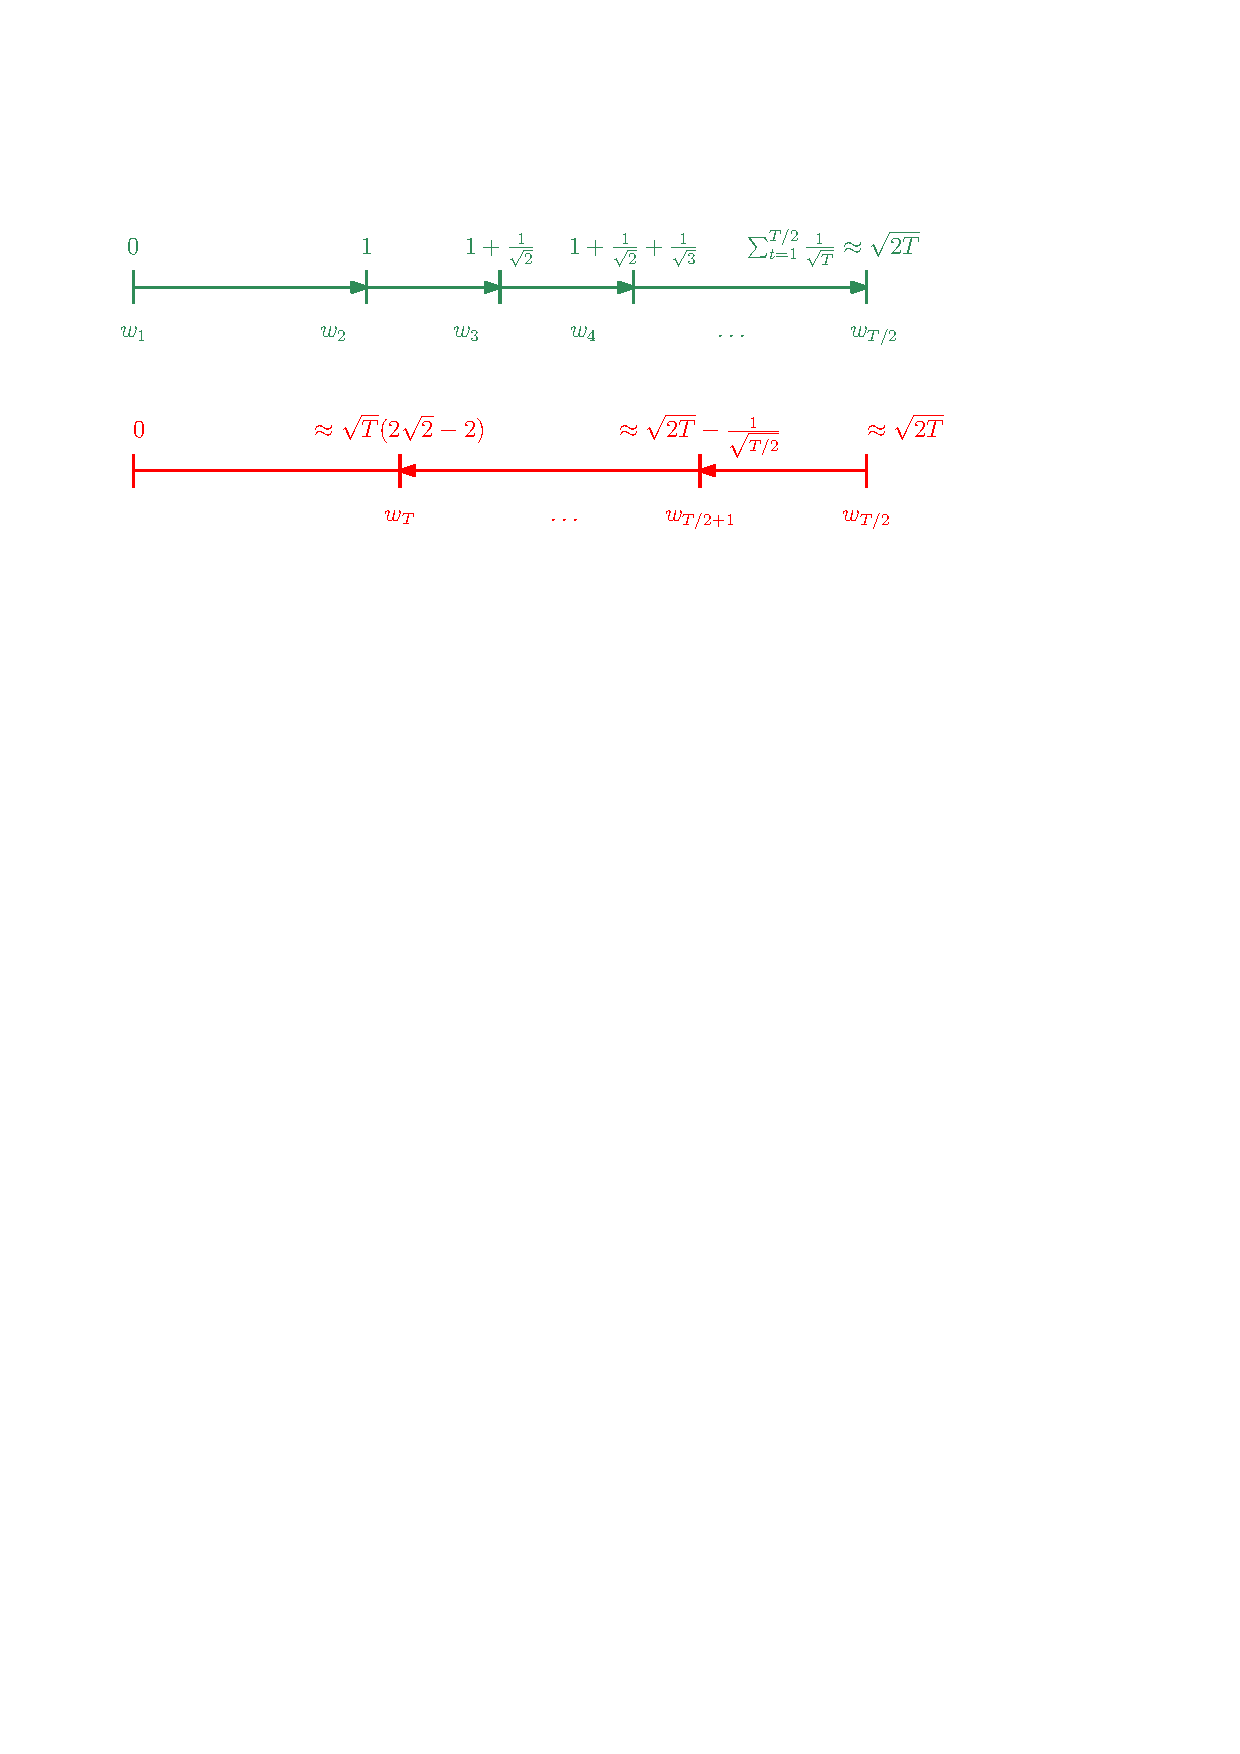
\includegraphics[scale=0.5]{gd-lower-bound}
\end{center}
$$
\Regret_T(0) = \sum_{t=1}^T w_t \ell_t = \textcolor{ForestGreen}{-\sum_{t=1}^{T/2} w_t} \quad \textcolor{Red}{+ \sum_{t={T/2+1}}^T w_t} \ge \frac{T^{3/2}}{20}
$$
\end{frame}

%%%%%%%%%%%%%%%%%%%%%%%%%%%%%%%%%%%%%%%%%%%%%%%%%%%%%%%%%%%%%%%%%%%%%%%%%%%%%%%%%%%%%%%%%%
\begin{frame}
\centering
\Huge
\textcolor{Blue}{Parameter-Free Algorithms}
\end{frame}

%%%%%%%%%%%%%%%%%%%%%%%%%%%%%%%%%%%%%%%%%%%%%%%%%%%%%%%%%%%%%%%%%%%%%%%%%%%%%%%%%%%%%%%%%%
\begin{frame}
\frametitle{Parameter-Freeness Problem}

\begin{theorem}
If $\norm{\ell_t}_* \le 1$ then FTRL/MD with learning rate $\eta$ satisfies
$$
\forall u \in K \qquad  \Regret_T(u) \le \frac{R(u)}{\eta} + \eta T \; .
$$
\end{theorem}

\pause

\vspace{0.5cm}

If we choose $\eta = \sqrt{R(u)/T}$,
$$
\Regret_T(u) \le 2 \sqrt{R(u) T} \; .
$$

\pause

\vspace{0.5cm}

Is there an \textbf{single} algorithm such that
$$
\forall u \in K \qquad \Regret_T(u) \le 2 \sqrt{R(u) T} \quad ?
$$
\end{frame}



%%%%%%%%%%%%%%%%%%%%%%%%%%%%%%%%%%%%%%%%%%%%%%%%%%%%%%%%%%%%%%%%%%%%%%%%%%%%%%%%%%%%%%%%%%
\begin{frame}
\frametitle{Parameter-Freeness: Experts}

$K=\Delta_N$ and $R(u) = \KL{u}{\tfrac{\textbf{1}}{N}}$

\pause
\vspace{1cm}

With learning rate $\eta = \sqrt{\frac{\ln N}{T}}$
$$
\forall u \in \Delta_N \qquad \Regret_T(u) \le \sqrt{T \ln N}
$$

\pause
\vspace{1cm}

Ideally, we want
$$
\forall u \in \Delta_N \qquad
\Regret_T(u) \le \sqrt{T \cdot \KL{u}{\tfrac{\textbf{1}}{N}}}
$$
\end{frame}

%%%%%%%%%%%%%%%%%%%%%%%%%%%%%%%%%%%%%%%%%%%%%%%%%%%%%%%%%%%%%%%%%%%%%%%%%%%%%%%%%%%%%%%%%%
\begin{frame}
\frametitle{Parameter-Freeness: Unconstrained Optimization}

$K=\R^N$ and $R(u) = \frac{1}{2} \norm{u}_2^2$

\pause
\vspace{0.5cm}

With learning rate $\eta = 1/\sqrt{T}$,
$$
\forall u \in \R^N  \qquad \Regret_T(u) \le \left(1 + \norm{u}_2^2 \right) \sqrt{T} \; .
$$

\pause
\vspace{0.5cm}

With learning rate $\eta = D/\sqrt{T}$,
$$
\forall u : \norm{u}_2 \le D \qquad  \Regret_T(u) \le D \sqrt{T} \; .
$$

\pause
\vspace{0.5cm}

Ideally, we want
$$
\forall u \in \R^N \qquad  \Regret_T(u) \le \norm{u} \sqrt{T} \; .
$$
\end{frame}

%%%%%%%%%%%%%%%%%%%%%%%%%%%%%%%%%%%%%%%%%%%%%%%%%%%%%%%%%%%%%%%%%%%%%%%%%%%%%%%%%%%%%%%%%%
\begin{frame}
\frametitle{Parameter-Free Algorithm for $\R^N$}

\fontsize{10pt}{14}\selectfont

Suppose $\norm{\ell_t}_2 \le 1$

\vspace{1cm}

\begin{tabular}{c|c}
\begin{minipage}{4.3cm}
\begin{algorithmic}
{
\STATE $L_0 \leftarrow 0$
\STATE $W_0 \leftarrow 1$
\FOR{$t=1,2,3,\dots$}
\STATE $w_t \leftarrow - \frac{W_{t-1}}{t}  L_{t-1} $
\STATE Predict $w_t$
\STATE Observe $\ell_t \in \R^N$
\STATE $L_t \leftarrow L_{t-1} + \ell_t$
\STATE $W_t \leftarrow W_{t-1} - \langle \ell_t, w_t \rangle$
\ENDFOR
}
\end{algorithmic}
\end{minipage}
&
\pause
\begin{minipage}{5.7cm}
\begin{itemize}
\item FTRL
\begin{itemize}
\item regularizer $R(u) = \frac{1}{2}\norm{u}_2^2$
\item learning rate $\eta_t = \frac{W_{t-1}}{t}$
\end{itemize}
\item Wealth $W_t = 1 - \sum_{i=1}^t \langle \ell_i, w_i \rangle$
\end{itemize}
\end{minipage}
\end{tabular}

\end{frame}

%%%%%%%%%%%%%%%%%%%%%%%%%%%%%%%%%%%%%%%%%%%%%%%%%%%%%%%%%%%%%%%%%%%%%%%%%%%%%%%%%%%%%%%%%%
\begin{frame}
\frametitle{Coin-Betting Algorithm}

\fontsize{10pt}{14}\selectfont

Coin flips $c_t \in \{+1,-1\}$

\vspace{0.5cm}

\begin{tabular}{c|c}
\begin{minipage}{4.3cm}
\begin{algorithmic}
{
\STATE $L_0 \leftarrow 0$
\STATE $W_0 \leftarrow 1$
\FOR{$t=1,2,3,\dots$}
\STATE $w_t \leftarrow W_{t-1} \frac{L_{t-1}}{t} $
\STATE Predict $w_t$
\STATE Observe $c_t \in \{+1,-1\}$
\STATE $L_t \leftarrow L_{t-1} + c_t$
\STATE $W_t \leftarrow W_{t-1} + c_t w_t$
\ENDFOR
}
\end{algorithmic}
\end{minipage}
&
\begin{minipage}{5.7cm}
\pause
\begin{itemize}
\item Wealth
$$
W_t = 1 + \sum_{i=1}^t c_i w_i
$$

\item Krichevski-Trofimov estimator
$$
\frac{L_{t-1}}{t} = \frac{\sum_{i=1}^{t-1} c_i}{t}  \in (-1,+1)
$$

\item Wealth satisfies
$$
W_t \ge \exp \left( t \cdot \KL{\frac{1}{2} + \frac{\sum_{i=1}^t c_i}{T}}{\frac{1}{2}} \right)
$$
\end{itemize}
\end{minipage}
\end{tabular}
\end{frame}

%%%%%%%%%%%%%%%%%%%%%%%%%%%%%%%%%%%%%%%%%%%%%%%%%%%%%%%%%%%%%%%%%%%%%%%%%%%%%%%%%%%%%%%%%%
\begin{frame}
\frametitle{Regret Bound}

\begin{theorem}
For convex function $F:K \to \R$,
$$
\forall u \in K \quad \Regret_T(u) \le F(u)
\quad \Longleftrightarrow \quad
- \underbrace{\sum_{t=1}^T \langle \ell_t, w_t}_{\Reward_T} \rangle \ge F^* \left(\sum_{t=1}^T \ell_t \right) \; .
$$
\end{theorem}
\pause
\vspace{-0.5cm}
$$
\underbrace{-\sum_{t=1}^T \langle \ell_t, w_t \rangle}_{\Reward_T}
= W_t - 1
\ge \underbrace{\exp \left( T \cdot \KL{\frac{1}{2} + \frac{\norm{\sum_{t=1}^T \ell_t}}{T}}{\frac{1}{2}} \right) - 1}_{F^*(\sum_{t=1}^T \ell_t)}
$$

\pause

\begin{theorem}
$$
\Regret_T(u) \le 1 + \norm{u}_2 \sqrt{T \ln\left(1 + 4T^2 \norm{u}_2^2 \right)}
$$
\end{theorem}

\end{frame}

%%%%%%%%%%%%%%%%%%%%%%%%%%%%%%%%%%%%%%%%%%%%%%%%%%%%%%%%%%%%%%%%%%%%%%%%%%%%%%%%%%%%%%%%%%
\begin{frame}
\frametitle{Results for Experts}

\begin{itemize}
\item $O(N)$ time per update and $O(N)$ memory, and
$$
\Regret_T(u) \le \sqrt{T \cdot \left(1 + \KL{u}{\tfrac{\textbf{1}}{N}} \right)} \; .
$$

\item $O(N \log \log N)$ time and memory, and
$$
\Regret_T(u) \le \sqrt{ \sum_{t=1}^T \norm{\ell_t}_\infty^2 \cdot \left(1 + \KL{u}{\tfrac{\textbf{1}}{N}} \right)} \; .
$$
\end{itemize}
\end{frame}

%%%%%%%%%%%%%%%%%%%%%%%%%%%%%%%%%%%%%%%%%%%%%%%%%%%%%%%%%%%%%%%%%%%%%%%%%%%%%%%%%%%%%%%%%%
\begin{frame}
\frametitle{Open Problems}

\begin{enumerate}
\item For given $K$ and a norm, construct non-negative $1$-strongly convex
function $R:K \to \R$ that minimizes
$$
\sup_{u \in K} R(u).
$$

\item For what $K$ and $1$-strongly convex $R:K \to \R$ can we have
$$
\forall u \in K \qquad \Regret_T(u) \le \sqrt{T \cdot R(u)} ?
$$

\begin{itemize}
\item Does $K$, $R$, $\Breg_R(\cdot,\cdot)$ need to be bounded?
\end{itemize}

\item What is the trade-off for unconstrained optimization?

\begin{itemize}
\item There is \textbf{no} algorithm that is simultanesouly scale-free
and parameter-free \Cite{Cutkosky-Boahen}.
\end{itemize}

\item $O(N)$ time and memory, parameter-free and scale-free algorithm
for experts (and combinatorial optimization).
\end{enumerate}

\end{frame}

\end{document}
